\chapter[2021 July]{July 2021}

\section[2021/07/03]{Saturday, 3 July 2021}

\subsection{End-Effector Mechanism}

\subsubsection{Rotary Motor Selection Considerations}

The rod designed to facilitate the rotation and linear buffer motion of the vacuum pad was further developed. Intuitively, the rod requires a relatively low amount of torque to initiate and maintain rotary motion. Therefore, the smallest class of \ac{NEMA} stepper motors, namely \ac{NEMA} 8 motors, were considered as a guide for the motor footprint in the mechanical design. A preliminary decision to use a stepper motor over a servo was made based on the fact that rotary stability is essential once the vacuum pad has reached its required orientation. Servo may pulsate at standstill which is undesirable as the gripped cube may displace adjacent cubes. Furthermore, the rotation speed requried is low and stepper motors exhibit the best torque characteristics at low speed. Lastly, in full step mode, NEMA 8 stepper motors typically exhibit a full step resolution of $1.8 ^\circ / \text{step}$ which falls within the rotatry accuracy specifications of $5 ^\circ$.

\subsubsection{Transmission Gear Design}

The width and breadth of the front face of the \ac{NEMA} 8 stepper motor is 20 mm and 20 mm. The diameter of the designed rotary rod is 13 mm. In order to facilitate a sufficient space between the motor and the rotary rod for spring and rotary rod gear, the centres of rotation of the rotary rod and the \ac{NEMA} 8 stepepr motor were placed 20 mm apart. Since the step accuracy of the motor is sufficient, no gearing ratio is required. Therefore, the most space efficent manner of connecting these two rotary centres is with two gears both with a pitch diameter of 20mm each. Since this is not a specialised application of these gears, relatively standard parameters were seleected for their design. The gear parameters as designed in Fusion 360 and used for both gears are as follows:

\begin{compactitem}
    \item Pressure Angle = $20 ^\circ$
    \item Module = 1
    \item Number of Teeth = 20
    \item Backlash = 0.3 mm
    \item Root Fillet Radius = 0.3 mm
    \item Pitch Diameter = 20 mm
\end{compactitem}

A relatively large backlash of 0.3 mm was selected due to the high tolerance required by 3D printed parts. A pressure angle of $20 ^\circ$ and $25 ^\circ$ are the most commonly used angles in gear design. A smaller pressure angle has weaker teeth but runs quieter. Due to the low torque nature of this gear application, a $20 ^\circ$ pressure angle was selected to take advantage of the qualitative low noise benefit.

\subsubsection{Torque Calculations}

The point of entry for calculating the various mass elements that need to be translated and rotated is the aluminium cube that needs to be manipulated. The density of aluminium is $2.7 g/cm^3$. Since the cube has a maximum side length of $1.3 cm$, the cube has a maximum mass of $5.94 g$. Using the updated design of the end-effector rod, the 3D model was converted to a triangle mesh and exported to the 3D printing slicer Cura. Using PLA 1.75mm filament, Cura estimated the weight of the part to be 7g when printed at 50\% infill. The following is a summary of the masses of the components that comprise the rotating mass in the end-effector as well as the mass of the cube gripped by the end-effector:

\begin{compactitem}
    \item Aluminium cube mass = 5.94 g
    \item 3D printed rotary rod at 50\% infill = 7 g
    \item ZPT08UN-B5 vacuum pad = 6 g
    \item M-5AU-6 barbed connector = 1.8 g
    \item Total mass = 20.74 g
\end{compactitem}

The system does not have any explicit angular velocity and angular acceleration specifications that it is required to meet from the project proposal. Therefore, it is decided that on a qualitative basis that the end-effector should be capable of completing a single rotation once every 4 seconds when at maximum velocity. Similarly, it is also decided that the end-effector should be capable of reaching this speed in 0.5 seconds from standstill. The angular velocity is computed as shown below in \EquRef{eqn:angular-velocity}.

\begin{align}
    \omega&=\frac{\Delta \theta}{\Delta t}
    \label{eqn:angular-velocity} \\
    \omega&=\frac{2\pi}{4}=\frac{\pi}{2} \text{ rad/s}
\end{align}

The maximum angular acceleration the motor should be capable of driving is as calculated in \EquRef{eqn:angular-acceleration} below assuming that the system accelerates linearly to the maximum velocity from standstill.

\begin{align}
    \alpha&=\frac{\Delta \omega}{\Delta t} 
    \label{eqn:angular-acceleration} \\
    \alpha&=\frac{\pi / 2 - 0}{0.5 - 0}=\frac{\pi}{4} \text{ rad/s}^2
\end{align}

In order to calculate the torque required to rotate the end-effector component, the moment of inertia $I_O$ about the centre of rotation $O$ of the component needs to be computed. The component is modelled as a cylinder with a radius of 10 mm and all of its mass located in its outer shell only. This is the cylindrical configuration that has the greatest moment of inertia and therefore requires the greatest torque to rotate. This guarantees that a motor capable of rotating this is capable of rotating the actual component. The moment of inertia for the cylindrical model is calculated as shown in \EquRef{eqn:moment-of-inertia} below

\begin{align}
    I_O&=mr^2
    \label{eqn:moment-of-inertia} \\
    I_O&=(20.74 \times 10^{-3})(20 \times 10^{-3})^2=8.296 \times 10^{-6} \, kg\cdot m^2
\end{align}

where $m$ is the mass of the cylinder and $r$ is the radius of the outer shell of the cylinder. In order to relate the kinematic motion of the rotary end-effector component to the external forces applied to it, the moment equation for rotation about a fixed axis $O$ shown in \EquRef{eqn:moment-equation} below can be used

\begin{align}
    \sum M_{Oi} = I_O \alpha
    \label{eqn:moment-equation} \\
    \sum F_i r_i = I_O \alpha
\end{align}

where $M_{Oi}$ is the moment that results from the application of force $F_i$ at the $i^{th}$ point at perpendicular distance $r_i$ from the axis of rotation $O$. Two external forces to the rotary end-effector component are considered, namely the force of static friction $F_{fs}$ and the force $F_A$ applied to the component gear by the gear on the motor's drive shaft. Only static friction is considered as it is generally greater than kinetic friction and therefore more challenging to overcome. The coefficient of static friction for plastic on plastic used in these calculations is $\mu _s = 0.4$. Furthermore, it is assumed that the friction only acts along the outer edge of the cylinder model since this is requires the most torque to overcome. $F_{fs}$ is computed as shown in equation \EquRef{eqn:static-friction} below

\begin{align}
    F_{fs}=\mu _s \times F_N
    \label{eqn:static-friction}
\end{align}

where $F_N$ is the normal force from the weight of the end-effector component on the bottom support. Using \EquRef{eqn:moment-equation}, the force required to accelerate the end-effector component from standstill at the required rate can be calulated as shown in \EquRef{eqn:Fa-required}

\begin{align}
    &F_A r_A - F_{fs} r_{fs} = I_O \alpha
    \label{eqn:Fa-required} \\
    &F_A (10 \times 10^{-3}) - [(0.4)(20.74 \times 10^{-3})(9.81)] (10 \times 10^{-3}) = (8.296 \times 10^{-6})\left(\frac{\pi}{4}\right) \\
    &F_A = 82.04 \times 10^{-3} \, N
\end{align}



\subsubsection{Rod and Motor Integration}

% \FigRef{fig:end-effector-integrated} shows the design of the updated rod design integrated with a NEMA 8 

% \begin{figure}[!ht]
%     \centering
%     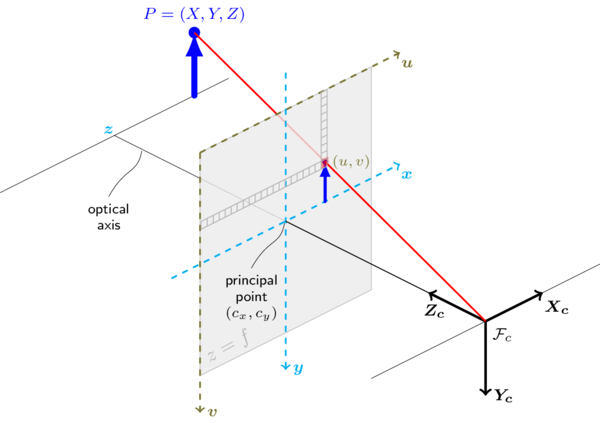
\includegraphics[width=0.7\linewidth]{figures/202107/pinhole-camera-model.png}
%     \caption{}
%     \label{fig:end-effector-integrated}
% \end{figure}



\pendsign